\documentclass[a4paper,10pt, twoside]{report}
\usepackage[utf8x]{inputenc}
\usepackage[T1]{fontenc}
\usepackage{titlesec, blindtext, color}
\usepackage{setspace}

\usepackage[hidelinks]{hyperref}

\usepackage{float}
\usepackage{fancyhdr}
\usepackage{graphicx}
\usepackage[top=2cm, bottom=3cm, left=2.5cm, right=2.5cm]{geometry}

\usepackage[french]{babel}

\pagestyle{fancy}
\setlength{\headheight}{49pt}
\setlength{\footskip}{17pt}
% header
\fancyhead[R]{
\includegraphics[width=5cm]{logo_sciences.png}}
\fancyhead[L]{
\includegraphics[width=5cm]{logo_arksens.png}}

% footer
\fancyfoot[C]{Rapport de stage --- Master 2 FSIL\\Ludovic Lubeigt}
\fancyfoot[RO, LE] {\thepage}

\definecolor{gray73}{gray}{0.73}
\newcommand{\hsp}{\hspace{20pt}}
\titleformat{\chapter}[hang]{\Huge\bfseries}
{\thechapter\hsp\textcolor{gray73}{|}\hsp}{0pt}{\Huge\bfseries}

\graphicspath{{images/}}

\begin{document}
\begin{spacing}{1.2}
 
% Page de garde
\begin{titlepage}
  \newgeometry{top=2cm, bottom=2cm, left=2cm, right=2cm}
  
  \begin{center}
    
\includegraphics[width=9cm]{logo_sciences.png}\\[2cm]
    
    \textsc{\bfseries\Large Rapport de stage\\[0.3cm]
    Master 2 -- Fiabilit\'e, S\'ecurit\'e et
    Int\'egration Logicielle\\[0.3cm]
        Parcours Fiabilit\'e et S\'ecurit\'e Informatique}\\[0.3cm]

    \rule{\linewidth}{1mm} \\[1cm]

    \textsc{\bfseries\huge Conception \&  d\'eveloppement syst\`eme de backup
    chiffr\'e et incr\'emental en C/C++}\\[1cm]

    \rule{\linewidth}{1mm}\\[1.5cm]

    \textsc{\huge Arksens Cyber Security}\\[2cm]
    
    \begin{figure}[H]
      \begin{minipage}[t]{8cm}
        \centering
        
\includegraphics[scale=0.50]{logo_adhara.png}
      \end{minipage}
      \begin{minipage}[t]{8cm}
        \centering
        
\includegraphics[width=7cm]{logo_arksens.png}
      \end{minipage}\\[1.3cm]
    \end{figure}
      
    \begin{minipage}{0.4\textwidth}
      \begin{flushleft} \large
        \emph{\bfseries Auteur :}\\
        Ludovic \textsc{Lubeigt}
      \end{flushleft}
    \end{minipage}
    \begin{minipage}{0.4\textwidth}
      \begin{flushright}
        \large \emph{\bfseries Tuteur Entreprise :}\\
        Ga\"etan \textsc{van Diemen}\\[0.2cm]
        \emph{\bfseries Enseignant :}\\
        Jean-Luc \textsc{Massat}
      \end{flushright}
    \end{minipage}\\[1.5cm]
      
    \large\emph{\bfseries Ann\'ee Universitaire :}\\
    2014 -- 2015

  \end{center}
\end{titlepage}

\begin{abstract}

Ce document pr\'esente le travail r\'ealis\'e lors du stage de fin d'\'etude
\`a Arksens Ltd. \`a l'\^ile Maurice entre le premier avril 2015 et le 25
septembre 2015 dans le cadre du Master 2 Fiabilit\'e et S\'ecurit\'e
Informatique \`a l'Universit\'e d'Aix-Marseille.

Le rapport est d\'ecoup\'e en deux parties. Une premi\`ere servant de rapport
de synth\`ese et pr\'esentant l'entreprise, le sujet de stage, le
travail effectu\'e de m\^eme que l'environnement de travail et les \'eventuelles
difficult\'es rencontr\'ees.
La seconde partie apporte un aspect technique au rapport et permet de 
pr\'esenter le travail r\'ealis\'e plus en d\'etail.
\end{abstract}

\newpage
\hfill
\section*{Remerciements}
Je tiens tout d'abord \`a remercier l'\'equipe p\'edagogique de la facult\'e des
sciences de l'universit\'e d'Aix-Marseille qui m'a permis d'avoir les
connaissances et les aptitudes n\'ecessaires au bon d\'eroulement de ce stage.

Je remercie \'egalement la soci\'et\'e Arksens pour m'avoir permis de faire mon
stage chez eux. Tout particuli\`erement, je remercie David Terranova et Ga\"etan
van Diemen qui m'ont accueilli \`a l'\^ile Maurice et suivi au jour le jour
durant ces six mois. Je n'oublie \'evidemment pas Micha\"el Colaone et le reste
de l'\'equipe pour l'accueil et la bonne ambiance au sein de l'entreprise.

Enfin je remercie toute les personnes que je peux oublier mais qui m'ont aid\'e,
dans l'\'ecriture de ce rapport, dans le cadre du stage ou qui m'ont tout
simplement fait d\'ecouvrir l'\^ile Maurice.

Je tiens tout particuli\`erement \`a remercier Sir Daniel Brands of House Brands,
the first of His Name, King of the Dutch, King of the flatlands and the first
Men, Breaker of Cars and Father of the Bikers.

\hfill
\tableofcontents
\thispagestyle{fancy}

\chapter*{Introduction}
\thispagestyle{fancy}
Dans le cadre du Master professionnel \textit{Fiabilit\'e, S\'ecurit\'e et
Int\'egration logicielle}, parcours \textit{Fiabilit\'e et S\'ecurit\'e
Informatique} \`a l'\textit{Universit\'e d'Aix-Marseille}, un stage de fin
d'\'etude doit \^etre effectu\'e en entreprise pour valider les acquis et
rentrer dans le monde professionnel.

J'ai r\'ealis\'e ce stage entre le 1\up{er} avril et le 25 septembre 2015, soit
une p\'eriode de six mois, \`a \textit{Adhara Cyber Security}, renomm\'ee 
\textit{Arksens} au 1\up{er} juillet.

Ce stage fut donc l'occasion pour moi de mettre en pratique mes connaissances,
acquises tout au long de mon parcours universitaire, dans un environnement
professionnel et de m'en servir pour mener au mieux la mission qui m'a
\'et\'e confi\'ee. En outre, j'ai d\^u cr\'eer \`a partir de rien un syst\`eme
de backup incr\'ementale et s\'ecuris\'e, offrant une encryption en local des
donn\'ees des utilisateurs. Ainsi m'a-t-il \'et\'e demand\'e de faire la
conception de ce projet dans un premier temps puis son d\'eveloppement dans un
second temps et ainsi voir le processus de cr\'eation, jusqu'\`a un stade
avanc\'e, de ce qui peut \^etre qualifi\'e de gros projet.

Ce rapport vient donc pr\'esenter le d\'eroulement du stage ainsi que le
travail accompli au sein de l'entreprise durant ces six mois.


\chapter{Rapport de synth\`ese}
\thispagestyle{fancy}
\section{Pr\'esentation de l'entreprise}
Cr\'e\'ee en 2013 et nomm\'ee alors \textit{Adhara Cyber Security} avant
d'\^etre renomm\'ee \textit{Arksens} au 1\up{er} juillet 2015, l'entreprise 
dans laquelle j'ai effectu\'e mon stage est sp\'ecialis\'ee en s\'ecurit\'e
informatique. se d\'eveloppe sur trois continents gr\^ace \`a une approche
novatrice et r\'epondant aux besoins des entreprises et administrations de
toutes tailles.

Le changement de nom a fait suite \`a une \'evolution des clients puisque
l'entreprise, bien que principalement prestataire de service pour des PME
s'est ouverte aux entreprises de taille plus importante. Revoyant leur
strat\'egie de commercialisation et de communication, l'entreprise se devait
donc de changer de nom.

Aujourd'hui \textit{Arksens} est donc pr\'esent dans trois pays se trouvant
chacun sur un continent diff\'erent (voir figure~\ref{mapArksens}). On retrouve
ainsi :
\begin{itemize}
  \item Abu Dhabi aux \'Emirats Arabes Unis pour les activit\'es au Moyen
  Orient.
  \item Pamplemousses à l’\^ile Maurice pour les activit\'es africaines.
  \item Paris en France pour les activit\'es européennes.
\end{itemize}

\begin{figure}[h!]
  \centering
  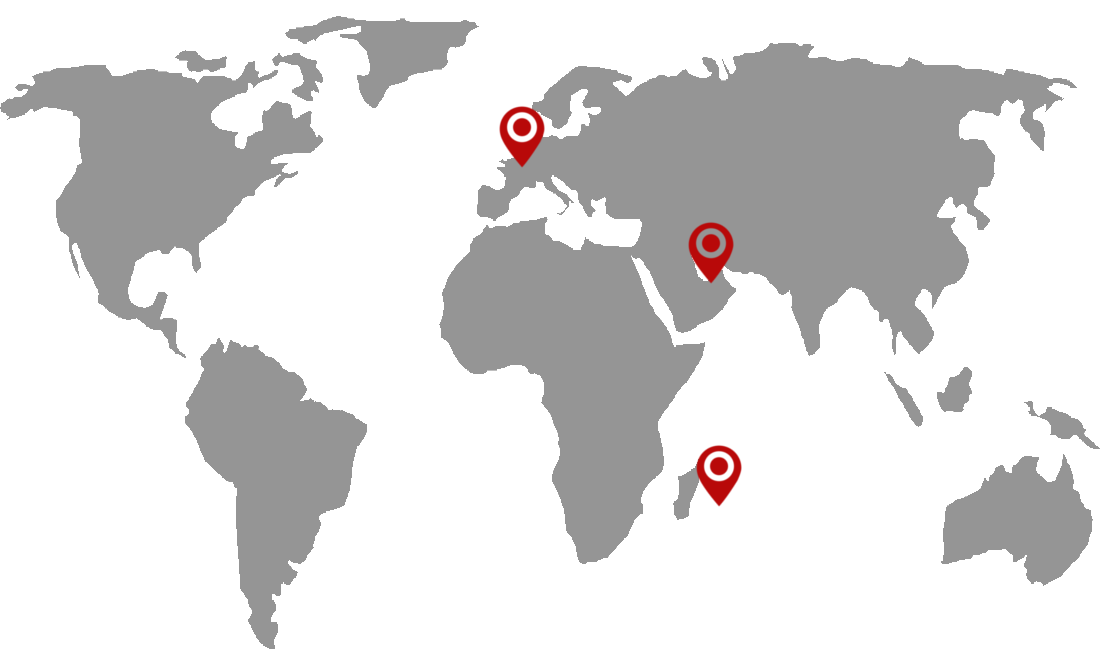
\includegraphics[scale=0.30]{map_arksens.png}
  \caption{\label{mapArksens} O\`u trouver Arksens}
\end{figure}
      
L'entreprise offre ainsi aux utilisateurs un service client de proximit\'e.
Pour ma part, c'est l'\^ile Maurice qui m'int\'eresse puisque c'est l\`a o\`u
j'ai pass\'e ces six mois de stage. Pamplemousses se trouve \`a proximit\'e
de Port Louis. Les locaux se trouvent au Business Park de Beau Plan
(figure~\ref{beauPlan}) \`a Pamplemousses, ville situ\'ee au nord de l'\^ile,
\`a proximit\'e de Port Louis. Les locaux accueillent donc le centre de
recherche et d\'eveloppement de l'entreprise.

\begin{figure}[h!]
  \centering
  \includegraphics[width=15cm]{beau_plan_soir.jpg}
  \caption{\label{beauPlan} Beau Plan Business Park}
\end{figure}

L'\'equipe a beaucoup \'evolu\'ee entre mon arriv\'ee et mon d\'epart puisque
seulement trois personnes en plus du PDG, Micha\"el Colaone, \'etaient
pr\'esentent au 1\up{er} avril, date de d\'ebut du stage : David Terranova,
directeur des op\'erations, Ga\"etan van Diemen, chef de projet ainsi que
Daniel Brands, d\'eveloppeur web arriv\'e quelques jours auparavant.

L'\'equipe s'est agrandie par deux fois. D'abord \`a la mi-avril avec
l'arriv\'ee de deux autres stagiaire, Didier Mannone et
Yves Colin de Verdi\`ere, puis au 1\up{er} mai avec l'arriv\'ee d'Aymeric
Tabourin, ing\'enieur s\'ecurit\'e.

L'int\'egration dans l'\'equipe fut donc facile et rapide et c'est donc dans
une bonne ambiance qu'a p\^u se d\'erouler ce stage de fin d'\'etude.

\end{spacing}
\end{document}          